\section{Approach}
\label{sec:approach}

Figure~\ref{} shows the high-level overview of our approach. Our approach
includes three major phases: capture, minimize, and explore. In the
capture phase, our approach records dynamic traces from program executions.
Our approach next transforms these dynamic traces into
PUTs and unit tests. As the dynamic traces are recorded from program
executions, we identify that there many duplicate traces as same 
sequence of method calls can get invoked multiple times. Consequently,
the generated PUTs and unit tests also include duplicates.
In the minimize phase, we use a combination of static and dynamic
analyses to filter out duplicate PUTs and unit tests, respectively.
In the explore phase, we use dynamic symbolic execution to explore
PUTs to generate unit tests that achieve a high code coverage
of the code under test. We next explain each phase in detail.

%------------------------------------------------------------------------
\subsection{Capture Phase}
\label{sec:capture}

The capture phase records dynamic traces from program executions. The capture
phase uses a profiler that records method calls invoked by the application
during execution. The capture phase records both method calls and the concrete
values passed as arguments to these method calls. Figure~\ref{fig:dynamictrace} shows
an example dynamic traces recorded by our capture phase. Statement 2
shows the concrete value \CodeIn{<\%\@ Page..u000a} passed as an argument
for the \CodeIn{Match} method call. The traces are recorded
are complete in the sense that these traces do not require any non-primitive
object types. Furthermore, method calls inside traces can be both
observer and state-modifying methods. TODO: Write definitions 
of observer and state-modifying method. 

\begin{figure}[t]
\begin{CodeOut}
\begin{alltt}
01: TagRegex tagex = new TagRegex();
02: Match mc = ((Regex)tagex).Match("<\%\@ Page..u000a",108);
03: Capture cap = (Capture) mc;
04: int indexval = cap.Index;
\end{alltt}
\end{CodeOut}\vspace*{-3ex}
\Caption{\label{fig:dynamictrace} An example dynamic trace recorded by 
the capture phase.}\vspace*{-3ex}
\end{figure}

The capture phase transforms recorded dynamic traces into PUTs and unit
tests. To generate PUTs, our approach identifies all values of primitive
types and promote those values as parameters. Furthermore, our approach identifies
return values of observer methods in the method-call sequence and
promotes them as \CodeIn{OUT} parameters for the PUT. In C\#, these
\CodeIn{OUT} parameters represent the return values of a method.
Our approach next generates a unit test that includes all concrete values
promoted as parameters. Figure~\ref{fig:putut} shows a PUT and an unit test
generated from the dynamic trace shown in Figure~\ref{fig:dynamictrace}.

\begin{figure}[t]
\begin{CodeOut}
\begin{alltt}

\emph{PUT:}
00: public static void $F_1$(string $VAL_1$, 
01: \hspace*{0.3in}int $VAL_2$, out int $OUT_1$) \{
02:    TagRegex tagex = new TagRegex();
03:    Match mc = ((Regex)tagex).Match($VAL_1$, $VAL_2$);
04:    Capture cap = (Capture) mc;
05:    $OUT_1$ = cap.Index;
06: \}

\emph{Unit test:}
07: public static void $T_1$() \{
08:      int index;
09:      $F_1$("<\%@ Page..u000a", 108, out index);     
10: \}

\end{alltt}
\end{CodeOut}\vspace*{-3ex}
\Caption{\label{fig:putut} A PUT and an unit test generated
from the dynamic trace in Figure~\ref{fig:dynamictrace}.}\vspace*{-3ex}
\end{figure}

The generated PUT includes two parameters and one \CodeIn{OUT} parameter.
The \CodeIn{OUT} parameter is the return value for the observer
method \CodeIn{Capture.Index}. These \CodeIn{OUT} parameters are later
helpful in capturing the actual values returned and can be used
for regression testing (Section~\ref{}). The figure also shows an unit
test generated from the dynamic trace. The unit test includes concrete
values of the dynamic trace and invokes the PUT with these concrete values.

%------------------------------------------------------------------------
\subsection{Minimize Phase}
\label{sec:minimize}

In our approach, we record dynamic traces during program executions. As the same
sequence of method calls can be invoked multiple times during program execution,
we identify that there are many duplicates among recorded dynamic traces.
Consequently, there are many duplicates among generated PUTs and unit tests. 
We next try to filter out duplicate PUTs and unit tests because using
dynamic symbolic execution for exploring these PUTs is redundant and also
may lead to scalability issues.

\begin{figure*}[t]
\centering
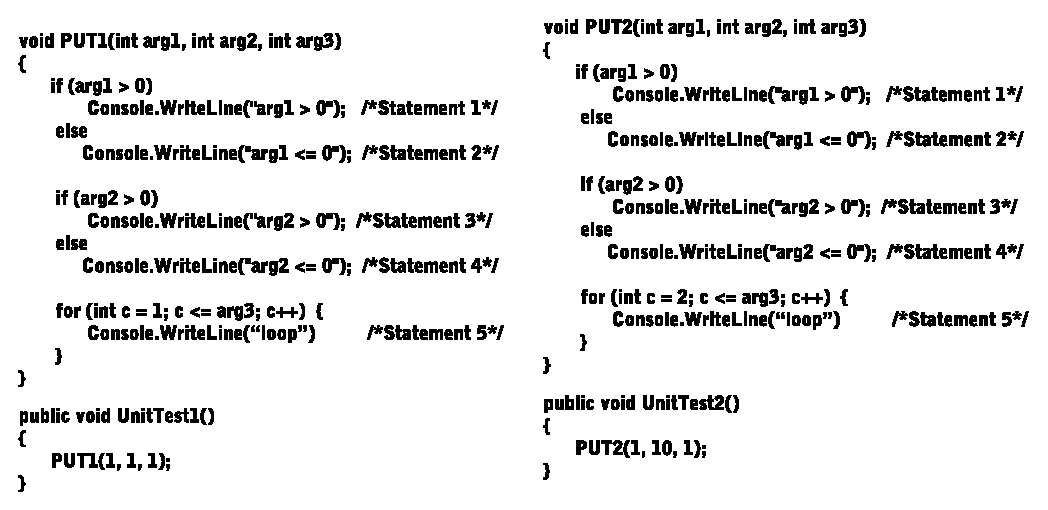
\includegraphics[scale=0.75,clip]{figs/PUTsAndUT1.eps}\vspace*{-1ex}
\caption{Two PUTs and associated unit tests generated by the capture phase.} \label{fig:samplePutAndUT}
\end{figure*}

We next describe how our approach filters out duplicate PUTs and unit tests using
illustrative examples shown in Figure~\ref{}. The figure shows three PUTs
and three unit tests generated from dynamic traces. We next describe how we filter
out duplicate PUTs and later explain how we filter out duplicate unit tests.

In our approach, we use static analysis for filtering out duplicate PUTs.
Consider two PUTs \CodeIn{PUT1} and \CodeIn{PUT2} shown in Figure~\ref{fig:samplePutAndUT}.
Our approach considers a PUT as a duplicate of another PUT if both PUTs include
the same sequence of instructions. Our approach compares instruction-by-instruction and checks whether both PUTs
are the same or not. Our approach ignores any primitive values related to local
variables in these PUTs while comparing instructions. 
In this example, our approach considers \CodeIn{PUT2} is a duplicate of \CodeIn{PUT1},
although the local variable \CodeIn{c} in Statement 5 is assigned different values.
As \CodeIn{PUT2} is a duplicate of \CodeIn{PUT1}, our approach automatically replaces
the method call for \CodeIn{PUT2} in \CodeIn{UnitTest2} with \CodeIn{PUT1}.

Our approach next uses dynamic analysis for filtering out duplicate unit tests.
Our approach considers a unit test as a duplicate of another unit test if both
unit tests exercise the same execution path. To detect duplicate unit tests,
our approach executes each unit test and monitors the execution path followed
by the unit test. For example, \CodeIn{UnitTest1} follows the path ``1 $\rightarrow$ 3 $\rightarrow$ 5''.
Our approach considers \CodeIn{UnitTest2} as a duplicate of \CodeIn{UnitTest1}, as \CodeIn{UnitTest2}
also follows the same path ``1 $\rightarrow$ 3 $\rightarrow$ 5'' in \CodeIn{PUT1}. 
Consider another unit test \CodeIn{UnitTest3} shown in Figure~\ref{fig:nonduplicate}.
Our approach does not consider \CodeIn{UnitTest3} as a duplicate test of \CodeIn{UnitTest1}
as \CodeIn{UnitTest3} follows the path ``1 $\rightarrow$ 3 $\rightarrow$ 5 $\rightarrow$ 5'',
since this unit test iterates the loop twice. TODO: To write some sentences
to show why we use more strict and precise analysis based on path coverage.
TODO: Do we need to explain more deeper on how we compute hash value for the
paths followed?

\begin{figure}[t]
\begin{CodeOut}
\begin{alltt}
public void UnitTest3() \{
\hspace*{0.5in}TestMe(5, 8, 2);
\}
\end{alltt}
\end{CodeOut}\vspace*{-3ex}
\Caption{\label{fig:nonduplicate} An example non-duplicate unit test.}\vspace*{-3ex}
\end{figure}

%------------------------------------------------------------------------
\subsection{Explore Phase}
\label{sec:explore}

TODO: Cite Patrice NDSS paper here for seed tests here.
In the explore phase, our approach uses Pex to explore PUTs and generate unit
tests. During this phase, we use existing tests as seed tests to increase the effectiveness
of our approach. TODO: To explain more of how the seed tests help increase the effectiveness of
DSE here. 

Pex generated $86$ regression unit tests for the PUT shown in Figure~\ref{fig:putut}. 
Figure~\ref{fig:generatedtests} shows the three sample regression tests generated by Pex.
In unit tests 1 and 2, Pex automatically annotated the unit tests with the expected exceptions
\CodeIn{ArgumentNullException} and \CodeIn{ArgumentOutOfRangeException}, respectively.
As the PUT includes an \CodeIn{OUT} parameter, Pex automatically added assertions
based on actual values captured while generating the unit test. These regression tests
can help expose the defects in later versions of Pex.

\begin{figure}[t]
\begin{CodeOut}
\begin{alltt}

\emph{Generated Test 1:}
00: [PexRaisedException(typeof(ArgumentNullException))]
01: public static void $F_102$() \{
02:     int i = default(int); 
03:     $F_1$ ((string)null, 0, out i);
04: \}

\emph{Generated Test 2:}
00: [PexRaisedException(typeof(ArgumentOutOfRangeException))]
01: public static void $F_110$() \{
02:     int i = default(int);
03:     $F_1$("", 1, out i);
04: \}

\emph{Generated Test 3:}
00: public static void $F_103$() \{
01:     int i = default(int);
//TODO: Uncomment the following line
\Comment{02:     $F_1$ ("\0\0\0\0\0\0\0<\u013b\0", 7, out i);} 
03:     PexAssert.AreEqual<int>(0, i);
04: \}

\end{alltt}
\end{CodeOut}\vspace*{-3ex}
\Caption{\label{fig:generatedtests} Regression tests generated by Pex by exploring 
the PUT shown in Figure~\ref{fig:putut}.}\vspace*{-3ex}
\end{figure}

Although Pex is effective in exploring PUTs and generating unit tests,
we identify that Pex or other symbolic execution tools can lead to scalability issues
when handling large number of PUTs. To address this issue, our approach uses
a distributed setup where Pex can be executed simultaneously on several machines.
Once started, our distributed setup is designed to run forever. The primary reason for such 
a setup is that it is hard to decide when to stop testing. Furthermore, to make sure that
exploration does not stuck with single PUT exploration, we use our distribution 
setup in a round-robin fashion. More specifically, our distributed setup runs
in iterations, where each iteration is bounded by parameters. For example, in the first
iteration, we use a timeout of three minutes for each PUT. We explore all PUTs with these
bounded parameters to generate unit tests. Once all PUTs are explored in one 
iteration, we double the parameters in the next iteration, where Pex can have more 
time to explore each PUT and achieve more code coverage. For example,
in second iteration, we use the timeout value as six minutes. 

To avoid Pex exploring same paths that were explored in previous iterations, we maintain
the database of seed tests. For example, all unit tests generated from Iteration 1 
are used as seed tests for Iteration 2. Using unit tests from Iteration 1 as seed
tests for Iteration 2 can help Pex explore quickly the new code regions.

